%% intro.tex
\chapter{Universal Tagger}
%%%%%%%%%%%%%%%%%%%%%%%%%%%%%%%%%%%%%%%%%%%%%%%%
\label{chap:uniTagger}

\section{Idea and Motivation} 
We have reviewed a possible approach for monolingual and multilingual POS tagger in the previous chapter. In this chapter, we aim to create our own universal tagger for many languages. Currently, there are separate taggers for many languages such as English, French, German, Italian, Arabic and so forth, where manually annotated data are available. \namecite{UniversalTagSet} show that the average accuracy for supervised learning for languages in table \ref{tab:tagAccuracySample} is as high as 95,2\% using the basic TNT tagger~\cite{TNTTagger}.  
\begin{table}
  \centering
    \begin{tabular}{llll}
    \textbf{Language} & \textbf{Source} & \textbf{\#Tags}  & \textbf{Accuracy} \\
	\hline
    Arabic & PADT/CoNLL07 & 21    & 96.1 \\
    Basque & Basque3LB/CoNLL07 & 64    & 89.3 \\
    Bulgarian & BTB/CoNLL06 & 54    & 95.7 \\
    Catalan & CESS-ECE/CoNLL07 & 54    & 98.5 \\
    Chinese & Penn ChineseTreebank & 34    & 91.7 \\
    Chinese & Sinica/CoNLL07 & 294   & 87.5 \\
    Czech & PDT/CoNLL07 & 63    & 99.1 \\
    Danish & DDT/CoNLL06 & 25    & 96.2 \\
    Dutch & Alpino/CoNLL06 & 12    & 93 \\
    English & PennTreebank & 45    & 96.7 \\
    French & FrenchTreebank & 30    & 96.6 \\
    German & Tiger/CoNLL06 & 54    & 97.9 \\
    German & Negra & 54    & 96.9 \\
    Greek & GDT/CoNLL07 & 38    & 97.2 \\
    Hungarian & Szeged/CoNLL07 & 43    & 94.5 \\
    Italian & ISST/CoNLL07 & 28    & 94.9 \\
    Japanese & Verbmobil/CoNLL06 & 80    & 98.3 \\
    Japanese & Kyoto4.0 & 42    & 97.4 \\
    Korean & Sejong & 187   & 96.5 \\
    Portuguese & Floresta Sint´a(c)tica/CoNLL06 & 22    & 96.9 \\
    Russian & SynTagRus-RNC & 11    & 96.8 \\
    Slovene & SDT/CoNLL06 & 29    & 94.7 \\
    Spanish & Ancora-Cast3LB/CoNLL06 & 47    & 96.3 \\
    Swedish & Talbanken05/CoNLL06 & 41    & 93.6 \\
    Turkish & METU-Sabanci/CoNLL07 & 31    & 87.5 \\
          & \textbf{Average} &       & \textbf{95.2 }\\
    \end{tabular}%
	 \caption{Tagging Accuracy of many languages using TNT }
  \label{tab:tagAccuracySample}%
\end{table}%
However, not many languages have enough labeled data to build a supervised tagger. Table \ref{tab:majorLanguageLessData}\footnote{source : http://www.ethnologue.org/ethno\_docs/distribution.asp?by=size} shows some major languages with no or very limited annotated data. However, with the growth of multilingual websites, government documents and large archives of human translation of books, news and so forth, unannotated parallel data is becoming more widely available. We believe that we can base on parallel data to build a bridge between languages and then copy tagging information from one language to another. This approach also exploits the idea that the tag ambiguity in one language is likely to correspond to an unambiguous word in other languages. Consider the example, ``\textit{we can can a can}" as in Figure \ref{fig:EnViparallel} and its Vietnamese translation ``\textit{Chung toi co the lam mot cai hop}". The ambiguous word ``\textit{can}" has several translations: ``\textit{co the}" (modal verb), ``\textit{lam}" (verb), ``\textit{cai hop}" (noun). Thus, the different translations help to disambiguate the syntactic category (POS tag) of word ``\textit{can}". Moreover, the underlining structure of a language can also be used to disambiguate. For example, in English, the word right after article is likely to be Noun or a capital word in German has a high chance to be Noun. Thus, the general idea of our Universal Tagger is exploiting the evidence from multiple languages via a parallel corpus. 
\begin{figure}
\centering
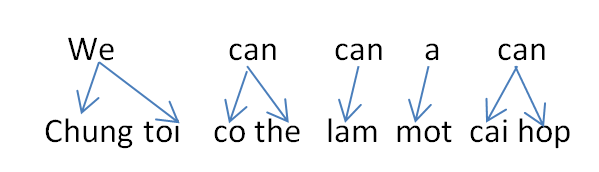
\includegraphics[scale=0.6]{Figures/EN_VI_SAMPLE}
\caption{English - Vietnamese parallel sentence}
\label{fig:EnViparallel}
\end{figure}

\begin{table}
  \centering
    \begin{tabular}{l|c}
    \textbf{Language} & \textbf{Native Speaker(millions)} \\
	\hline
	Bengali & 181 \\
    Javanese & 84.6 \\
    Lahnda & 78.3 \\
    Telugu & 70 \\
    Vietnamese & 69 \\
    Tamil & 65.7 \\
    ... & ...\\
    \end{tabular}%
	 \caption{Major languages with less annotated data 
	 }
  \label{tab:majorLanguageLessData}%
\end{table}%


\section{Universal Tagset}
The universal tagset is the tagset used for our universal tagger. One goal of universal tagger is to motivate the comparison between languages. Thus, universal tagset should be the common denominator of all languages. We adopt the work of \cite{UniversalTagSet} on 12 universal tags which is described in Table \ref{tab:univesalTagset}. We believe that this basic 12 tags are shared among most languages of the world. 
\begin{table}
  \centering
    \begin{tabular}{|c|p{12cm}|}
    \hline
	Tag & Description\\
	\hline \hline
	NOUN & nouns \\
	VERB & verbs\\
	ADJ & adjectives \\
	ADV & adverbs \\
	PRON & pronouns \\
	DET & determiner and articles \\
	ADP & preposition and postpositions\\
	NUM & numerals \\
	CONJ & conjuctions \\
	PRT & particles \\
	. & punctuation marks \\
	X & all other categories such as foreign word, abbreviation etc.\\
	\hline
    \end{tabular}
  \caption{12 tags of the Universal tagset  }    
  \label{tab:univesalTagset}%
\end{table}%
% Benefit of universal tagset 
The universal tagset benefits downstream applications that work across languages such as multilingual taggers, multilingual parsers and so forth. With the consensus tagset, the questions such as ``Tagging language A is harder than language B" would become easier to answer. Moreover, the universal tagger exploits the idea of projecting tag information from a resource-rich language to a resource-poor one. Adopting the universal tagset means that we do not need to care about matching between different tagsets. In addition, we do not have any official tagset for many widely spoken languages such as Telugu or Vietnamese. In this case, a universal tagset would be a good start. 

Nevertheless, we acknowledge that we are loosing information using universal tagset. For example, all \textit{VB, VBD, VBG, VBN, VBP, VBZ} tags from Penn treebank tagset are mapped to \textit{VERB} of Universal tagset. However, this is the trade-off we need to make. % Trade off of content 
\namecite{UniversalTagSet} also provided the mapping from many other tagsets to Universal tagset. Table \ref{tab:tagAccuracySample} lists all the available mapping from each language specific tagset to Universal tagset. In many languages the mapping is clear but in some languages it is not that obvious. \namecite{UniversalTagSet} shows an example of Korean where the adjective is missing. They use stative verb to describe the property of objects, hence, stative verb is mapped to \textit{ADJ} in universal tagset. The other example is the tagset used in French Treebank, there are no \textit{NUM} tags. Numbers are tagged as  adjective or nouns case by case. 
% Provide the mapping 
% Draw back of mapping

% TODO : Write automatic mapping here 
Normally, the mapping is done manually by a linguistic expert. However, \namecite{mapToUniversalTagset} also suggested methods to automatically map from language specific tagsets to the universal tagset. 

%%%%%%%%%%%%%% THIS IS TEMP PART, MERGE TO CH3 when finish 
\section{Methodology}

Here we describe our proposed tagger. The key idea is to maximize the
amount of information gleaned from the source language, while limiting
the amount of noise. Our approach contains 2 main steps (1) Building seed model (2) Apply self-training with revision. We describe the seed model and then explain how it is successively refined through self-training and revision.


\subsection{Seed Model}
\label{seedModel}

The first step is to construct a seed tagger from directly-projected
labels. Given a parallel corpus for a source and target language,
Algorithm~\ref{alg:seedmodel} provides a method for building an
unsupervised tagger for the target language. In typical applications,
the source language would be a resource-rich language having a
tagger, while the target language would be resource-poor, lacking a
tagger and large amounts of manually POS-labelled data.


\begin{algorithm}
\caption{Build seed model}
\label{alg:seedmodel}
\begin{algorithmic} [1]
\STATE Tag source side.
\STATE Word align the corpus with Giza++ and remove the many-to-1 mappings.
\STATE Project tags from source to target using the remaining 1-to-1 alignments.
\STATE Select the top $n$ sentences based on sentence alignment score.
\STATE Estimate emission and transition probabilities. 
\STATE Build seed tagger T. 
\end{algorithmic}
\end{algorithm}

Step 2 aligns words from source to target sentences. Words are aligned if they are translation of each other. There are cases where one word from source sentence is matched with exactly one word in the target sentence (one-to-one mapping) or one word in source sentence is mapped with a phrase in target sentence (many-to-one mapping). We eliminate many-to-one alignments (Step 2). Keeping these alignment would give
more POS-tagged tokens for the target side, but also introduce
noise. For example, suppose English and French were the source and
target language, respectively. In this case alignments such as English
\emph{laws (NNS)} to French \emph{les (DT) lois (NNS)} would be
expected \cite{YarowskyAndNgai} as shown in Figure \ref{fig:sampleEn_Fr}. However, in step 3, where tags are projected from the source to target language, If we just copy tag information from English side \textit{NNS} (common noun) to French side, both ``\textit{les}" and ``\textit{lois}" would be tagged as \textit{NNS}. However, this is incorrect for ``\textit{les}" which must be \textit{DT} (determiner). 

 \begin{figure}
 \centering
 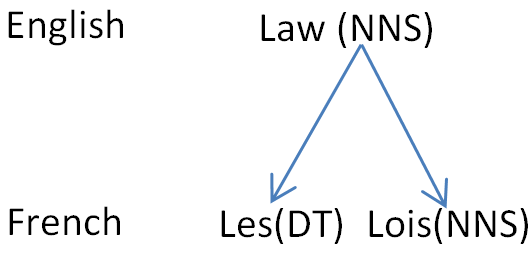
\includegraphics[scale=0.4]{Figures/En_Fr_sample.png}
 \caption{Many-to-one mapping case between English(law) and French(les lois)}
 \label{fig:sampleEn_Fr}
 \end{figure}


We build a French tagger based on English--French parallel data from the Europarl Corpus \cite{europarl}. We want to know the accuracy and coverage of the tags obtained through direct projection. We thus compare these tags again French Melt POS tagger~\cite{DBLP:DenisS09}. This is a supervised French tagger built on French treebank (FTB)~\cite{ftb}. They report the per-token accuracy is as high as 97.80\% and thus, a good approximation for our experiment. Table~\ref{tab:coverageAndAccuracy} confirms
that the one-to-one alignments indeed give higher accuracy but lower
coverage than the many-to-one alignments. One-to-one alignment covers 68\% of the token in French size (that is 32\% is unaligned). However, if we use both one-to-one and many-to-one mapping, we cover 20\% more of the tokens, but the accuracy is dropped by 10\% (absolute). It's worth noting that, accuracy is only calculated from aligned tokens.  Therefore, assuming that we have exactly 1000 tokens, if we used just one-to-one mapping, the number of correctly tagged tokens is $1000 \times 0.68 \times 0.78 = 530$ tokens. The number for additionally use many-to-one mapping is $1000 \times 0.88 \times 0.68 = 598$. That is we have $\frac{598 - 530}{1000} = 6.8$\% more accurately tagged tokens. However, many-to-one introduces more noise (as mentioned in Figure \ref{fig:sampleEn_Fr}), at this stage of the model we hypothesize that high-confidence tags are important, and hence we eliminate the many-to-1 alignments.

\begin{table}
  \small
\tabcolsep 5pt
  \centering
    \begin{tabular}{lcc}
    \hline
	Model & Coverage & Accuracy\\
	\hline 
	Many-to-1 alignments & 88\%& 68\% \\
	1-to-1 alignments    & 68\% & 78\%\\
	1-to-1 alignments: Top 60k sents   & 91\% & 80\%\\
	\hline
    \end{tabular}
  \caption{Token coverage and accuracy of many-to-1 and 1-to-1
    alignments, as well as the top 60k sentences based on alignment
    score for 1-to-1 alignments, using directly-projected labels
    only.}
  \label{tab:coverageAndAccuracy}%
\end{table}%


In Step 4, in an effort to again obtain higher quality target language
tags from direct projection, we eliminate all but the top $n$
sentences based on their alignment scores, as provided by the aligner
via IBM model 3.
%TODO : what is sentence alignment score is ???  How to calculate sentence alignment score ? 
We heuristically set this cutoff to 60k to balance the accuracy and size of the seed model\footnote{We considered values in the range 60--90k, but this choice had little impact on the accuracy of the model. Alternatively, we can set the threshold for sentence alignment score is $10^{-7}$}.
%% PC Is there anything more we can say about choosing the cutoff? Can we
%% briefly summarize the results using other cutoffs?
%% I add the foodnote 
Returning to our preliminary English--French experiments in
Table~\ref{tab:coverageAndAccuracy}, this process gives improvements
in both accuracy and coverage. In the top 60k sentence, we just retain 1-to-1 alignment. The coverage is improved from 68\% to 91\% and the accuracy is also improved from 78\% to 80\%. We also considered using both one-to-one and many-to-one alignments for the top 60k sentences, but in preliminary experiments this did not perform as  well, possibly due to the previously-observed problems with many-to-one alignments. Normally, the higher coverage, the lower accuracy and vice-versa, by simply ranking sentences and choose the first 60k, we have high coverage but in the same time, retain high accuracy. This is a \textit{crucial step} in our proposed methods. 
  
  
%% PC I don't think it's appropriate to be talking about overall accuracy
%% here, because it's confusing given that we're talking about a
%% different type of accuracy in table 1. What would the Coverage and
%% accuracy be for the top 60k sents for the many-to-one alignments?
%% PC I think we could drop this FN to save space.
The step 5 which is for estimating transition and emission probability is based on the following intuition. The number of parameters for the emission probability $p(w|t)$ is $|V| \times |T|$ where $w$ is word, $t$ is tag, $V$ is the vocabulary and $T$ is the tag set. The transition probability $p(t_i|t_{i-1}t_{i-2})$, on the other hand, has only $|T|^3$ parameters
for the trigram model we use. We use the universal tagset, thus, $|T|= 12$ but $|V| \approx 120k$ for French in a preliminary English-French experiment. Because of this huge difference in the number of parameters, in step 5, we employ different strategies to estimate the emission and transition probabilities. The emission probability is estimated from all 60k selected sentences. However, for the transition probability, which has less parameters, we again focus on ``better''
sentences, by estimating this probability from only those sentences
that have 
\begin{enumerate}
\item Token coverage $>90\%$ (based on direct projection of
from the source language)
\item Length $>4$ tokens
\end{enumerate}
These 2 criteria aim to identify longer, mostly-tagged sentences, which we
hypothesize are particularly useful as training data. The underlying reason is that we want to estimate transition probabilities with as small bias as possible. For example, the first token of a sentence is likely to be subject and therefore, \textit{Noun}. If we allow short sentences ($<= 3$ tokens) when calculating trigram transition probability, the model will favor the distribution which start with \textit{Noun}. This is undesirable for our model. In the same idea, a token missing inside a sentence disrupts the normal tag trigram distribution, thus, we reduce this by heuristically choosing only high coverage sentences ($>90$\%) . 


In the case of our preliminary English--French experiments, roughly 62\% of the 60k selected sentences meet these two criteria and are used to estimate the transition probabilities. For unaligned words, we simply assign a random POS and very low probability, which does not substantially affect transition probability estimates. 

In Step 6 we build a tagger by feeding the estimated emission and
transition probabilities into the TNT tagger \cite{TNTTagger}, an
implementation of a trigram HMM tagger.


\subsection{Self training and revision}
\label{selfTrainingAndRevision}
Up to this point we already have a tagger (seed model). In this section, we are going to improve this seed model by applying self-training with special revision. We exploit the large number of target language sentences available that have been
partially tagged through direct projection, in order to build a more
accurate tagger. Back to the preliminary English--French experiments, we just used 60k first sentence for the seed model, however, there are 1.9 millions other sentences. In this part, we are going to exploit the rest of data. 

Algorithm~\ref{alg:selfTraining} describes the
process of self training and revision, and assumes that the parallel
source--target corpus has been word aligned, with many-to-one
alignments removed, and that the sentences are sorted by alignment
score. In contrast to Algorithm~\ref{alg:seedmodel}, all sentences are
used, not just the 60k sentences with the highest alignment scores.

\begin{algorithm}
\caption{Self training and revision}
\label{alg:selfTraining}
\begin{algorithmic} [1]
\STATE Divide target language sentences into blocks of $n$ sentences.
\STATE Tag the first block with the seed tagger.
\STATE Revise the tagged block.
\STATE Train a new tagger on the tagged block.
\STATE Add the previous tagger's lexicon to the new tagger.  
\STATE Use the new tagger to tag the next block.
\STATE Goto 3 and repeat until all blocks are tagged.
\end{algorithmic}
\end{algorithm}

We believe that sentence alignment score might correspond to
the difficulty of tagging. By sorting the sentences by alignment score,
sentences which are more difficult to tag are tagged using a more
mature model.  Following Algorithm~\ref{alg:seedmodel}, we divide
sentences into blocks of 60k. As mentioned before, many-to-one mapping introduce noise, therefore, we just remove it here. 

 \begin{figure}
 \centering
 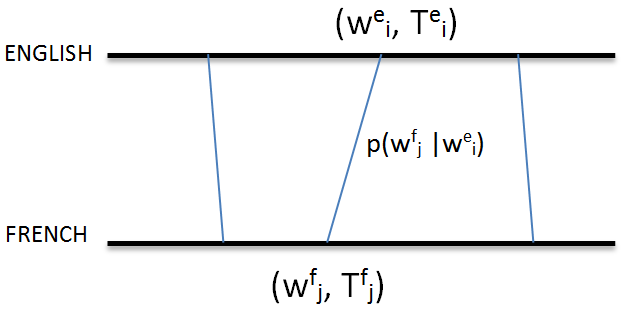
\includegraphics[scale=0.4]{Figures/English_French.png}
 \caption{Alignment between source(English) and target(French) language}
 \label{fig:alignment}
 \end{figure}

In step 3 the tagged block is revised by comparing the tags from the
tagger with those obtained through direct projection. Suppose source
language word $w^e_i$ is aligned with target language word $w^f_j$
with probability $p(w^f_j|w^e_i)$, $T^e_i$ is the tag for $w^e_i$
using the tagger available for the source language, and $T^f_j$ is the
tag for $w^f_j$ using the tagger learned for the target language as shown in Figure \ref{fig:alignment}. If $p(w^f_j|w^e_i) > S$, where $S$ is a threshold which we heuristically set to 0.7, we replace $T^f_j$ by $T^e_i$.  Self-training can suffer from over-fitting, in which errors in the original model are repeated and amplified in the new model \cite{McClosky:2006}.  To avoid this, we remove the tag of any token that the model is uncertain of, i.e.,
if $p(w^f_j|w^e_i) < S$ and $T^f_j \neq T^e_i$ then $T^f_j =
\mathrm{Null}$. So, on the target side, aligned words have a tag from
direct projection or no tag, and unaligned words have a tag assigned
by our model. By keeping the sentences in the order of difficulty to tag, the more we iterate, the more tokens are labeled by maturer model. It also means that, the more we iterate, we trust our model more and the direct projection less as shown in Figure \ref{fig:relianceTagger}. 

 \begin{figure}
 \centering
 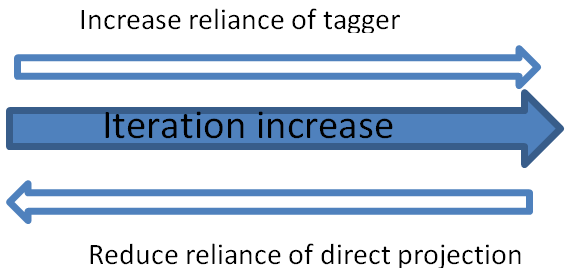
\includegraphics[scale=0.5]{Figures/iterationVsReliance.png}
 \caption{Reliance of tagger and direct projection label}
 \label{fig:relianceTagger}
 \end{figure}


Step 4 estimates the emission and transition probabilities as in
Algorithm~\ref{alg:seedmodel}. In Step 5, emission probabilities for
lexical items presented in the previous model, but missing from the current
model, are added to the current model. Later models therefore take
advantage of information from earlier models, and have wider coverage.

\section{Experiment Detail}
\label{sec:experimentDetail}


In this section, we are going to describe in detail our experiments. In the light of comparing with the state-of-the-art \cite{Das:2011}, we experiment in the way that result would be comparable. 

\subsection{Source data}
Using parallel data from Europarl \cite{europarl} we apply our method
to build taggers for the same eight target languages as
\namecite{Das:2011} --- Danish (da), Dutch (nl), German (de), Greek (el), Italian (it), Portuguese (pt), Spanish (es) and Swedish (sv) --- with English as the source language. \namecite{Das:2011} choose these 8 languages simply because the amount of parallel data for these languages is numerous. Europarl is the corpus collected from European Parliament date back to 1996. At that time, official languages for European Union are only 11 languages. Aside from 8 languages we chose, 3 others are English (en), Finnish (fi) and French (fr). From 2004, European Union expand to 25 members and more languages are added. Thus, due to the long history, the amount of data for these 8 languages we chose are superior compare with most of other languages. 

Our training data (Europarl) is a subset of the training data of
\namecite{Das:2011}, who also used the ODS United Nations dataset
which we were unable to obtain. Less data and as will be shown, the result are comparable, actually make this work stronger than the state-of-the-art. The overview of Europarl for all 8 languages is given in the Table \ref{tab:overviewEuroparl8Lang}. Aside from Greek which has approximately 1.2 million sentences, other language pairs have approximate 1.9 million sentences. 

\begin{table}[htbp]
  \centering

    \begin{tabular}{lrrr}

    \multicolumn{1}{c}{\textbf{Parallel Corpus (L1-L2)}} & \multicolumn{1}{c}{\textbf{Sentences}} & \multicolumn{1}{c}{\textbf{L1 Words}} & \multicolumn{1}{c}{\textbf{English Words}} \\\hline

    Danish-English & 1,968,800 & 44,654,417 & 48,574,988 \\
    Dutch-English & 1,997,775 & 50,602,994 & 49,469,373 \\
    German-English & 1,920,209 & 44,548,491 & 47,818,827 \\
    Greek-English & 1,235,976 & 32,031,068 & 31,929,703 \\
    Italian-English & 1,909,115 & 47,402,927 & 49,666,692 \\
    Portuguese-English & 1,960,407 & 49,147,826 & 49,216,896 \\
    Spanish-English & 1,965,734 & 51,575,748 & 49,093,806 \\
    Swedish-English & 1,862,234 & 41,508,712 & 45,703,795 \\

    \end{tabular}%
    \caption{Overview of Europarl dataset for 8 languages}  
    \label{tab:overviewEuroparl8Lang}%
\end{table}%

\subsection{Word alignment}
After collecting parallel data for each language, we are going to word align the data using the basic open source Giza++ to do the job. However before aligning, we should pre-process the data and pre-compute files needed for alignment. 

\subsubsection{Tokenize the sentence} This step aim at separating each token by a space. It is not as easy as it appear. Model should be able to handle the punctuation well. For example, period ``." which is used as sentence boundary should be separated but not in \textit{``Mr. Paul"} or \textit{``i.e"}. We use an open source \emph{tokenizer.perl} tool from Giza++ package to tokenize both source and target file.

\subsubsection{True casing}
True casing help to choose the most proper casing for each words. For example, the word beginning sentence should be uppercase. However, defining sentence boundary might be tricky. The usual heuristic ``." separate sentences is not always true. For example, ``." in the composition cases such as ``\textit{i.e.}" or ``\textit{Mr.}" does not mark sentence ending.
We also used an open source tool from Giza++ including two steps. (1) Train the model using \emph{train-truecaser.perl}   and (2) true casing using \emph{truecase.perl}. The first steps will output the true casing model which is used in the second step. 

%\begin{verbatim}
%train-truecaser.perl --model ModelFile --corpus input file
%truecase.perl --model ModelFile < input file > output file
%\end{verbatim}

\subsubsection{Cleaning}
Too long sentences are unreliable and not particularly suitable for our task. Therefore, we cut off sentence that longer than 80 words in both side of training data, using \emph{clean-corpus-n.perl} also from Giza++ package.  
%\begin{verbatim}
%clean-corpus-n.perl inPrefix file1 file2 outPrefix 1 80
%\end{verbatim}
%The command will cutoff sentence longer than 80 words from file \texttt{inPrefix.file1 } and \texttt{inPrefix.file2} to form two new files \texttt{outPrefix.file1} and \texttt{outPrefix.file2}. 
The above French-English parallel data from Europarl, approximately 43k (2.2\%) sentences are cutoff. 

\subsubsection{Getting vocabulary and bitext file}
Vocabulary file is needed to run Giza++. It lists the vocabulary and word's frequency in the training data. We must obtain vocabulary file for both source and target language. We use tool $plain2snt.out$ from Giza++ package to build vocabulary for both source and target langauge at once. 
\begin{verbatim}
plain2snt.out source target
\end{verbatim}
The output will be \texttt{source.vcb, target.vcb, source_target.snt, target_source.snt} The first 2 files are vocabulary files for source and target language. The next 2 files are bitext files which represent parallel sentence as  sequence of number. Each number is an id in the vocabulary file. Bitext files are also needed for word alignment. 
%The output will be vocabulary and bitext files for source and target language. Bitext files represent parallel sentence as  sequence of number. Each number is an id in the vocabulary file. Bitext files are also needed for word alignment. 


\subsubsection{Getting word classes}
Word-class files are used just for IBM-model 4/HMM. Syntactic and semantic similar words are grouped into classes. We make use of \emph{mkcls} tool. It's important that word class file name must comply with vocabulary file name. 
\begin{verbatim}
mkcls -psource -Vsource.vcb.classes
mkcls -ptarget -Vtarget.vcb.classes 
\end{verbatim}
%TODO : expand this part if you can 
\subsubsection{Word Alignment}
Everything needed to run word alignment is ready. There are many possible parameters, however, we use the default setting for this experiment. 
\begin{verbatim}
GIZA++ -S source.vcb -T target.vcb -C source_target.snt -o ALIGN
\end{verbatim}
Sometime, co-occurrence file is needed. This file can easily acquire using $snt2cooc.out$ tool. The output would have \texttt{ALIGN} prefix. There are many output files however, we particularly interested in (1) Lexical translation table file i.e. \texttt{ALIGN.t3.final}. (2) Alignment file i.e. \texttt{ALIGN.A3.final}. From these 2 files we will know the alignments and their confidence. Alignment is the most time consuming step in our whole process. To align each language pair in the Europarl corpus, it took us approximately a day on a eight core Intel Xeon 3.16 GHz CPU with 32 Gb Ram. The disadvantage of Giza++ is that, we can not achieve many-to-many mapping. That is, it always aligns from source to target, thus, just produce many-to-one and one-to-one mapping. We can fix this one by running Giza++ from other direction from target to source and merge two results. However, this step will double the running time. We will leave it for future work. 
% Disadvantage OK 

\subsection{Direct tag projection}
We tag the source file (English) with English Stanford POS Tagger \cite{Toutanova:2003}. This available tagger employs Penn treebank tagset which contain of 45 tags. Afterward, we use the mapping from \cite{UniversalTagSet} to map into Universal Tagset (12 tags). Then tags are copied from source side (English) to target side (foreign language) using just one-to-one alignment. 

\subsection{Seed model and final model}
\normalsize
We get sentence score from IBM model 3, that is, \texttt{ALIGN.A3.final}. Sentence score is used to rank sentence.  The following is the sentence pair getting from English-French Europarl parallel data. English sentence \emph{``resumption of the session"} is aligned with French sentence \emph{``reprise de la session"} with sentence alignment score = 0.006578. 


\scriptsize
\begin{lstlisting}
# Sentence pair (1) source length 4 target length 4 alignment score : 0.006578
reprise de la session 
NULL ({ }) resumption ({ 1 }) of ({ 2 }) the ({ 3 }) session ({ 4 }) 
\end{lstlisting}
\normalsize
First 60k sentences are used to build seed model which is described in section (\ref{seedModel}). Then, we use seed model to build final model by applying self-training and revision, section \ref{selfTrainingAndRevision}.

\subsection{Evaluation}
We used the same per-token accuracy evaluation metric as the state-of-the-art~\cite{Das:2011}. Test data for all 8 languages (Danish, Dutch, German, Greek, Italian, Portuguese, Spanish, Swedish) are also the same. These test data which is mainly come from CoNLL-X and CoNLL-07 share tasks. Table \ref{tbl:annotatedData} shows the source and size of test data for each language. We also use the mapping from \cite{UniversalTagSet} to map each language into Universal Tagset. 

\begin{table}
\small
\centering
    \begin{tabular}{lp{3cm}r}
    Language & Source & Number of Words \\
    \hline
    da       & DDT/CoNLL06& 94386           \\
    nl       & Alpino/CoNLL06& 203568          \\
    pt       & Floresta/CoNLL06& 206678          \\
    sv       & Talbanken/CoNLL06& 191467          \\
    el       & GDT/CoNLL07& 65419           \\
    it       & ISST/CoNLL07& 76295           \\
    es       & Cast3LB/CoNLL06& 89334           \\
    de       & Tiger/CoNLL06& 712332          \\
    \end{tabular}
    \caption{Size and source of annotated data}
    \label{tbl:annotatedData}
\end{table}

% List overview of data 
% Just use training data for this task
% Explain mapping process 

\section{Experimental Results}
We experiment as described in previous section \ref{sec:experimentDetail}. 
Using parallel data from Europarl \cite{europarl} we apply our method
to build taggers for the same eight target languages as
\cite{Das:2011} with English as the source language.  Our
training data (Europarl) is a subset of the training data of
\namecite{Das:2011}. The evaluation metric and test data
are the same as that used by \citeauthor{Das:2011}. Our results are
comparable to theirs, although our system is penalized by having less
training data. 

\begin{table}
\small
\tabcolsep 5pt
\begin{center}
\begin{tabular}{lcccccccccc}
        \hline
        ~                      & da & nl & de & el & it & pt & es & sv & & Avg. \\ \hline
        Seed model             & 83.7   & 81.1  & 83.6   & 77.8 & 78.6    & 84.9       & 81.4       & 78.9    & & 81.3   \\ 
        Self training + revision & \textbf{85.6}  & \textbf{84.0}    & \textbf{85.4}   & 80.4  & 81.4   & 86.3       &   83.3     & \textbf{81.0}      & & 83.4   \\ 
        \cite{Das:2011}          & 83.2   & 79.5  & 82.8   & \textbf{82.5}  & \textbf{86.8}    & \textbf{87.9}       & \textbf{84.2}    & 80.5    & & \textbf{83.4}   \\ 
\hline
Prop. of unknown words  & 10.9   & 10.7 & 10.6      & 6.0     & 12.8    & 9.6       & 8.0        & 7.3    & & 9.5   \\
        %% \hline
\end{tabular}
\caption{Token-level POS tagging accuracy for our seed model, self
  training and revision, and the method of \protect\cite{Das:2011}. The best results on each language, and on average, are shown in bold. }
\label{tab:taggingAcc}
\end{center}
\end{table}


Table~\ref{tab:taggingAcc} shows results for our seed model, self
training and revision, and the results reported by
\citeauthor{Das:2011}. Self training and revision improves the
accuracy for every language over the seed model, and gives an average
improvement of roughly two percentage points. The average accuracy of
self training and revision is on par with that reported by
\citeauthor{Das:2011}. On individual languages, self training and
revision and the method of \citeauthor{Das:2011} are split --- each
performs better on half of the cases. Interestingly, our method
achieves higher accuracies on Germanic languages --- the family of our
source language, English --- while \citeauthor{Das:2011} perform
better on Romance languages. This might be because our model relies on
alignments, which might be more accurate for more-related languages,
whereas \citeauthor{Das:2011} additionally rely on label propagation.

The last row of Table~\ref{tab:taggingAcc} shows the percentage of
unknown words for each language on the test data. On average,
approximately 10\% of the test data tokens are unknown. One way to
improve the performance of our tagger might be to reduce the
proportion of unknown words by using a larger training corpus, as
\citeauthor{Das:2011} did. We should also consider corpus that cover wider topics. Language used in Europarl is formal and domain specific such as news, politic, economic etc. However, test data covers many more subjects such as fiction, sport etc. That might be the reason why despite Europarl is a very huge corpus, unknown word (OOV) rate is still high. 


 \begin{figure}
 \centering
 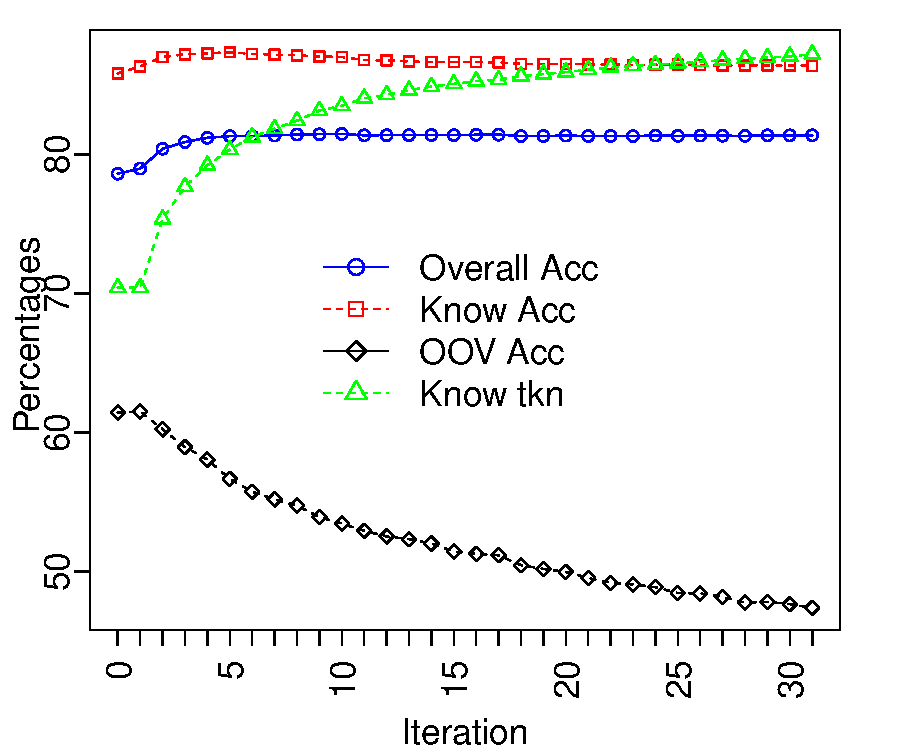
\includegraphics[scale=0.7]{Figures/itAcc}
 \caption{Overall accuracy, accuracy on known tokens, accuracy on
   unknown tokens, and proportion of known tokens for Italian.}
 \label{fig:italian}
 \end{figure}

Compared to \namecite{Das:2011}, our model performs poorest on
Italian, in terms of percentage point difference in accuracy.
Figure~\ref{fig:italian} shows accuracy,
accuracy on known words, accuracy on unknown words, and proportion of
known tokens for each iteration of our model for Italian. Iteration 0
is the seed model, and iteration 31 is the final model. Our model
performs poorly on unknown words as indicated by the low accuracy on
unknown words. The ``overall accuracy" line is always between ``known accuracy" and ``unknown accuracy" line weighted by ``proportion of known tokens" line. Thus, despite unknown words' accuracy drops drastically from 62\% to 47\%, an overall accuracy still (slightly) increases thank to increment on known accuracy words and proportion of known tokens. 

The poor performance on unknown words is expected because we do not use any language-specific rules to handle this case. Moreover, for the final model, approximately 13\% of the test data tokens are unknown.  This is the highest rate compare to other languages as in Table \ref{tab:taggingAcc}. This also partially explain why performance is poor on Italian. 

 \begin{figure}
 \centering
 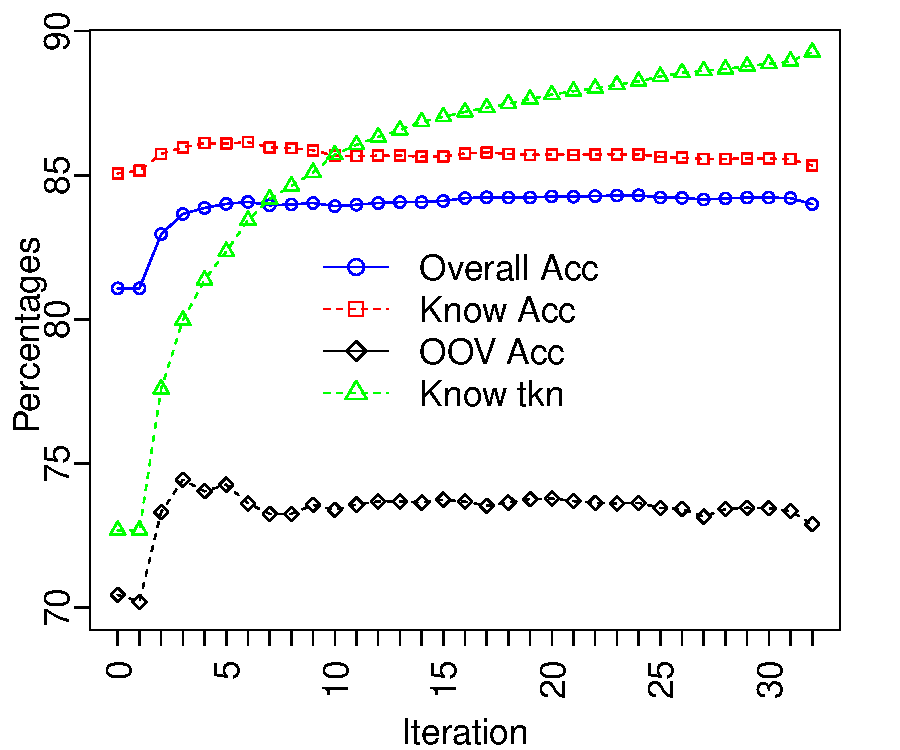
\includegraphics[scale=0.7]{Figures/nlAcc}
 \caption{Overall accuracy, accuracy on known tokens, accuracy on
   unknown tokens, and proportion of known tokens for Dutch.}
 \label{fig:dutch}
 \end{figure}

We examine the impact of self-training and revision over training
iterations. We find that for all languages, accuracy rises quickly in
the first 5--6 iterations, and then subsequently improves only
slightly. We exemplify this in Figure~\ref{fig:dutch} for Dutch, findings are similar for other languages. Although accuracy does not increase much in later iterations, they may still have some benefit as the vocabulary size continues to grow.

\section{Summary of Contributions}

We have proposed a method for unsupervised POS tagging (Universal tagger) that performs on par with the current state-of-the-art \cite{Das:2011}, but is substantially less-sophisticated (specifically not requiring convex 
optimization or a feature-based HMM). The complexity for fully optimizing a convex function is $O(n^3)$ where $n$ is size of data. This complexity is impractical because $n$ is very big ($n \approx $ 2 millions). \namecite{Das:2011} avoid this by just optimize for 10 iterations, instead of looping until converge. The complexity for each iteration is $O(n^2)$. So the overall complexity is $O(n^2)$. The complexity of our algorithm, on the other hand, is just $O(nlogn)$. This complexity is derived from sentence score sorting operation. The huge difference in complexity resulting in substantial running speed variance. We re-implemented label propagation from \cite{Das:2011}. It took over a day to complete this step on an eight core Intel Xeon 3.16 GHz CPU with 32 Gb Ram, but only 15 minutes for our model.  Moreover, unlike \namecite{Das:2011} who can not publish their code due to company license restriction, we made our code available for download\footnote{https://code.google.com/p/universal-tagger/} which hopefully will aid the development of multilingual natural language processing (NLP).

In future work we intend to consider using a larger training corpus to reduce the proportion of unknown tokens and improve accuracy. We can align source and target language in both directions, i.e.\ from source to target and from target to source language. Merging two alignment might yield a better one-to-one mapping set.

Given the improvements of our model over that of \citeauthor{Das:2011} on languages from the same family as source language, and the observation of
\namecite{SnyderMultilingualPOS} that a better tagger can be learned from
a more-closely related language, we also plan to consider strategies
for selecting more appropriate source language for a given target
language. 

Using our final model with unsupervised HMM inference methods might improve the final performance too, i.e.\ use our final model as the initial state for HMM, then experiment with different inference algorithms such as Expectation Maximization (EM), Variational Bayers (VB) or Gibbs sampling (GS). We in fact have tried EM, but it did not help. The overall performance dropped slightly. This might be because self-training with revision already found the local maximal point. However, VB or GS might help. \namecite{Gao:2008} compare EM, VB and GS for unsupervised English POS tagging. In many cases, GS outperformed other methods, thus we would like to try GS first for our model. 
